\begin{figure}
    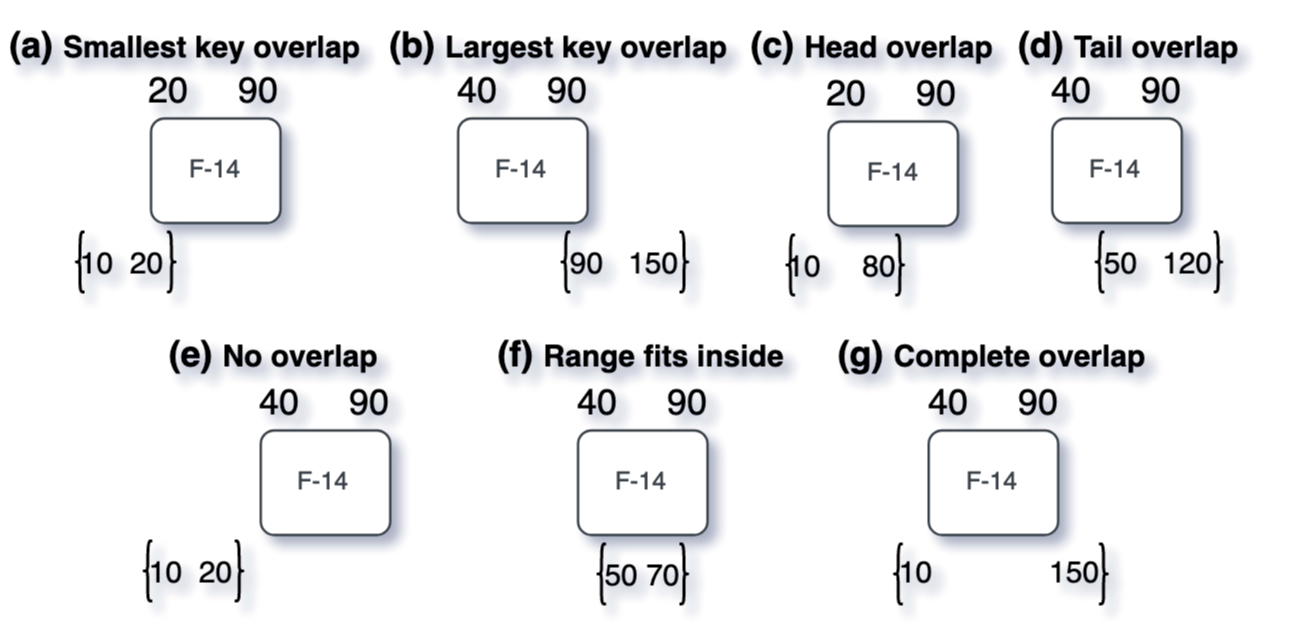
\includegraphics[scale=0.2]{Figures/File range overlaps.png}
    \caption{Possible file overlaps with range-query}\label{fig:file_range_overlaps}
\end{figure}

LSM-based data stores are designed to efficiently manage write-heavy workloads. The data is ingested through 
an in-memory buffer (a.k.a memtable in Rocksdb), a data structure that stores keys and their corresponding values. 
Once an in-memory buffer reaches its capacity, it is flushed to the disk in the form of an immutable sorted file (a.k.a Sorted Strings Table, SSTable or SST). 
These sorted files together forms a single sorted run which represents one level of LSM tree. Every level is completely sorted 
across all files, that are sorted by key. The compactions are triggered in the background when the size of a level exceeds a 
specific threshold.

\Paragraph{Updates in LSM} Updates are executed in an out-of-place fashion, where new values are written to lower levels 
while retaining old values in higher levels.

\Paragraph{Deletes in LSM} Deletions are performed by adding a special marker called a \textit{tombstone}. Tombstones are 
utilized to filter out logically deleted keys during range queries or compactions. They also serve as a form of soft 
deletion for point queries. Tombstones are removed when they reach the lowest level of the LSM structure.

\Paragraph{Range queries in LSM} LSM supports range queries by merging keys from multiple levels and filtering out 
invalid keys.

In the context of range queries, LSM-based data stores typically employ a straightforward approach: they create an 
iterator for each level and perform a K-way merge. This merge process involves pulling files sequentially or 
asynchronously from each level into memory and executing a sort-merge operation. The K-way merge eliminates the need 
to load all files from each level into memory simultaneously, thus reducing memory footprint.

\Paragraph{Leveled Compaction} Leveled compaction uses ``merge with'' strategy, where each level is merged with 
next level, which is usually much larger as per the configured size ratio.

The compactions are triggered to move data from lower levels to higher levels. The process involves selecting a file 
based on a compaction score from the lower level using a configured compaction policy. This file is then merged with 
overlapping files from the higher level. Invalid keys are filtered out during this merge, and the valid keys are 
written to the higher level. The compaction process will always occurs between adjacent levels. Once a file is compacted, 
it is removed from the lower level, and the new compacted file is written to the higher level. This process can repeat
multiple times until the level size falls below a specified threshold.

\begin{figure*}
    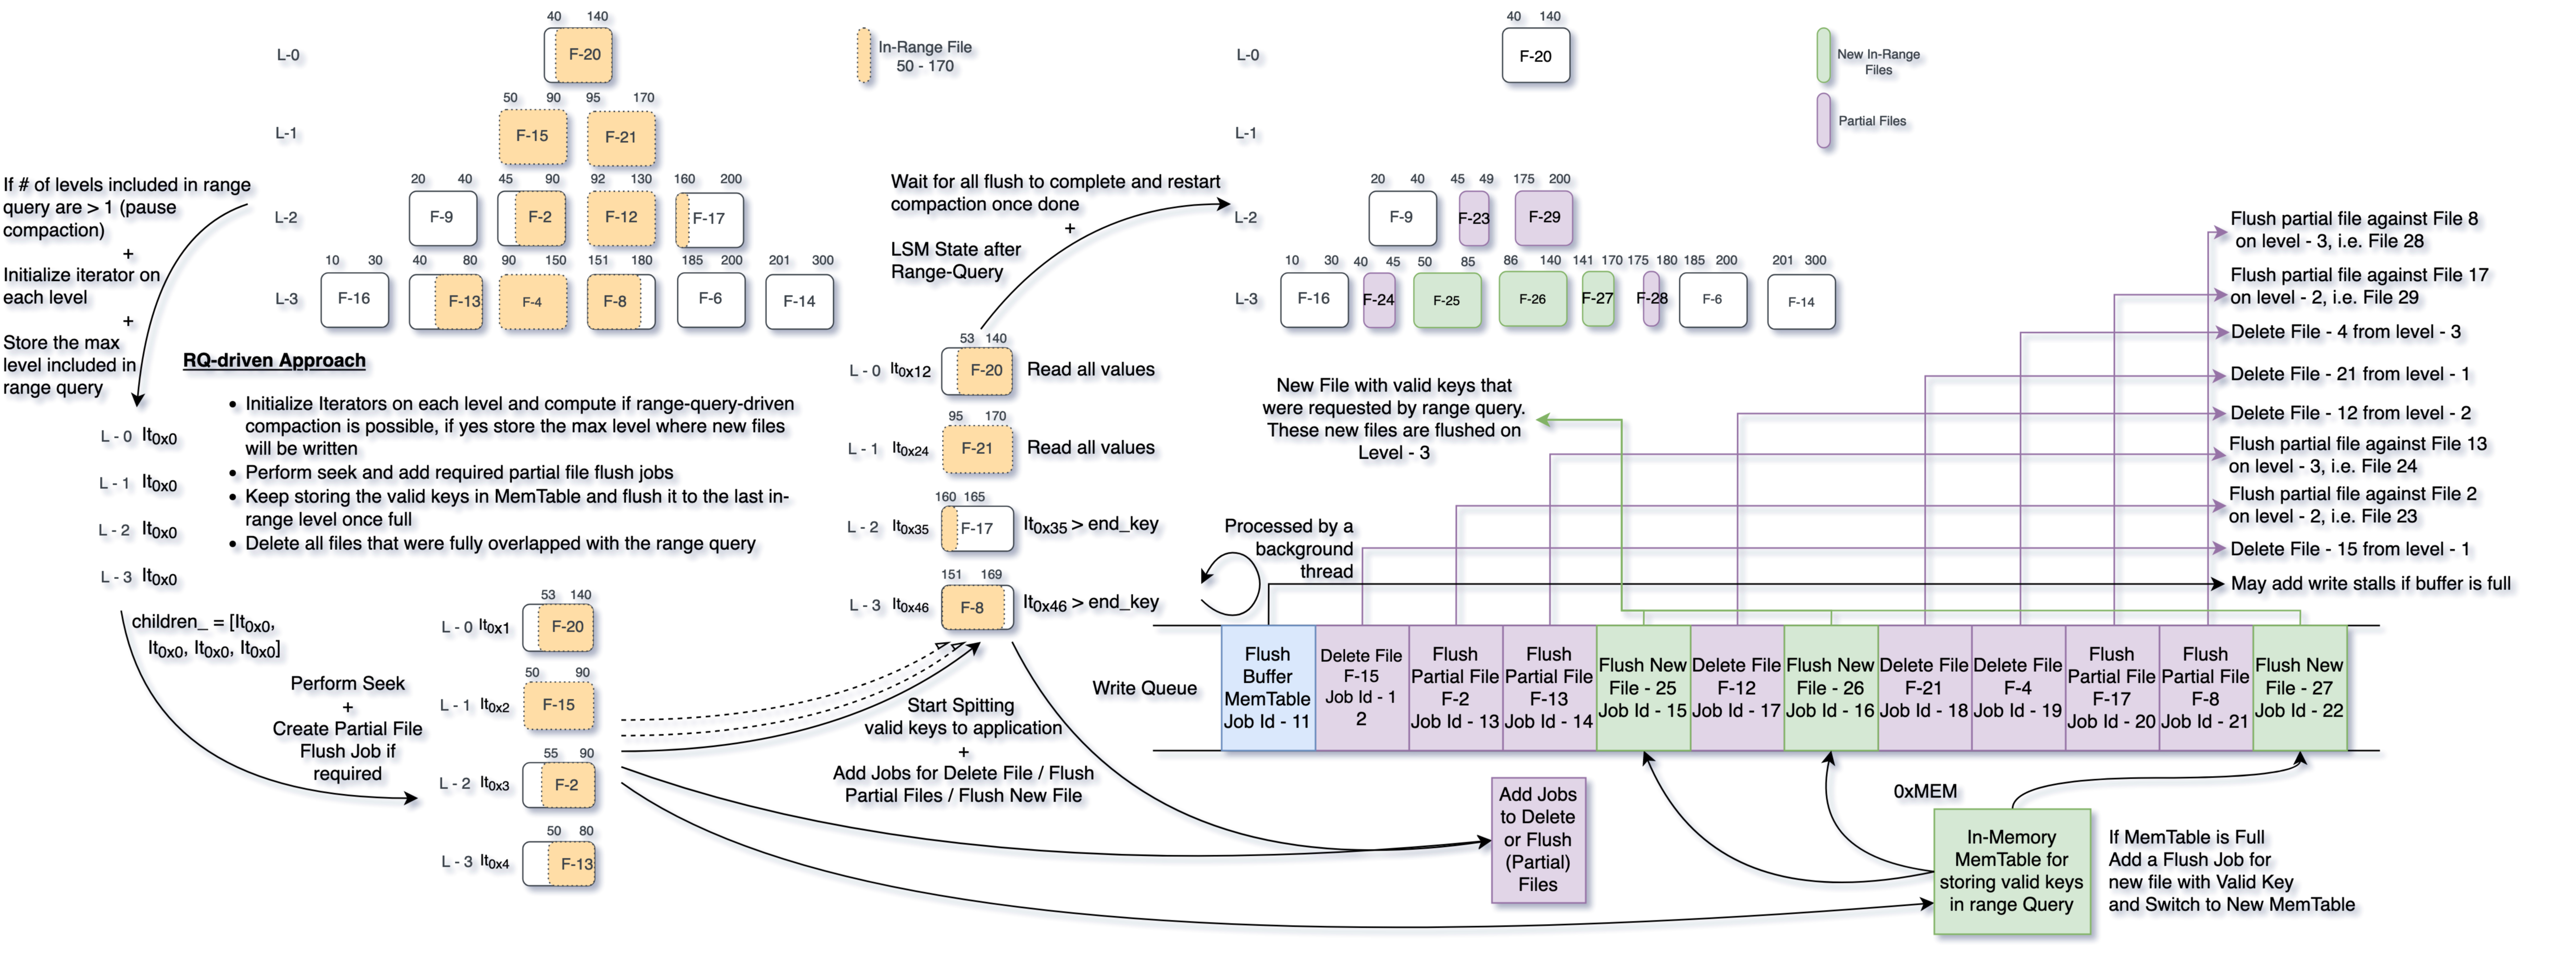
\includegraphics[scale=0.10]{Figures/RQ-driven numeric key sorting.png}
    \caption{Flow diagram of query-driven compaction in LSM. This outlines the steps involved in compaction during range query.}\label{fig:query-driven_compaction}
\end{figure*}